\capitulo{5}{Aspectos relevantes del desarrollo del proyecto}

En este capítulo vamos a destacar los puntos claves del proyecto y como se han llevado a cabo.

\section{Lenguaje para el desarrollo del proyecto}

Desde un primer momento se decidió el empleo de PHP como lenguaje central en la implementación del proyecto dado que permite el desarrollo web de contenido dinámico. El proyecto se ha llevado a cabo con Sublime Text, lo cual ha permitido una implementación del código más sencilla ya que iba mostrando posibles predicciones de texto.

PHP ha hecho posible aplicar alguna técnica de programación orientada a objetos, que se puede observar en el código del algoritmo de Backpropagation donde existen dos clases.
Se barajó la opción de implementar el código en Python y dejarlo embebido sobre PHP pero la idea inicial se descartó debido a que algunas funciones como las de acceso a la base de datos son únicas desde Drupal.

\subsection{PHP en Drupal}
La base de datos de MySQL estaba vinculada con Drupal, por lo que existe acceso desde Drupal a la base de datos. Para el acceso, el código PHP debía tener algunas sentencias exclusivas. La función db\_query tiene una sintaxis similar a las que se conocen ya que el contenido es una consulta MySQL sencilla. En cambio, otras funciones como db\_update, db\_select o db\_insert tienen una estructura completamente diferentes a las conocidas aunque son sencillas de utilizar.

Para poder desarrollar todo el código sobre Sublime Text y que no hubiese necesidad de copiarlo continuamente en los nodos de Drupal, fue necesario añadir un inclue\_once tanto en el nodo de Drupal como en el script.

\section{Datos de entrada a la red neuronal}
Es preciso darle un sentido a los datos que se han ido recopilando mediante los algoritmos de scraping, ya que el objetivo es darle a la red neuronal unos datos a partir de los cuales pueda ir aprendiendo y encontrar patrones. Son dos los algoritmos de scraping que fueron recopilando los datos que más tarde han sido empleados como entrada a la red Neuronal.

El primer algoritmo extrae todas las estadísticas de cada uno de los partidos de una jornada y los almacena en la base de datos. El segundo extrae la posición y las estadísticas de cada equipo en cada jornada, para almacenarlos posteriormente en la base de datos. A partir de estos datos recopilados se calculan las rachas de los equipos, donde se tiene en cuenta los puntos de cada equipo en las últimas jornadas acontecidas, los goles a favor y  los goles en contra. De esta forma se favorece al algoritmo para conocer la tendencia del equipo en las últimas jornadas. 

En el entrenamiento, por cada una de las instancias se le pasan al algoritmo un total de 78 columnas, donde las 30 primeras contienen los estadísticas del partido, de la 30 a la 54 las rachas y las estadísticas del equipo local en la clasificación y de la 54 a la 78 lo correspondiente al equipo visitante. Como función objetivo se establece 0 si ganó el equipo local, 1 si ganó el equipo visitante y 0.5 si el resultado final fue empate.
Antes de la entrada de los datos al algoritmo se realiza una normalización de los mismos respecto a la misma columna del resto de instancias, siendo la normalización:
\begin{center}
\large{$$v' = \frac{v-min_{a}}{max_{a}-min_{a}}$$}
\end{center}

En un primer momento se pensó introducir todos los partidos anteriores como instancias, independientemente el equipo hubiese disputado el partido como local o como visitante, para diferenciarlo se establecía un campo en la tabla \textit{clasificacion\_jornada}, llamado \textit{local\_visitante}, este campo se encuentra a 0 si el equipo juega como local o 1 si juega como visitante. Dado que los resultados obtenidos no eran óptimos se planteó otra posibilidad: si el equipo iba a disputar el partido como local se tomaban únicamente los datos de los partidos como local para ese equipo y para el rival lo mismo, se iban a tomar los datos como visitante.

Se realizó un estudio durante tres jornadas, en concreto las jornadas 12, 13 y 14, para elegir una de las opciones planteadas previamente. En las tablas \ref{tabla:jornada12}, \ref{tabla:jornada13} y \ref{tabla:jornada14} podemos observar los resultados obtenidos por los algoritmos. \textit{Pronóstico 1} es el primer método donde se utilizaban todos los partidos, mientras que el segundo método donde diferenciabamos local y visitante es \textit{Pronóstico 2}.

Una vez analizados los datos vemos como es el segundo método el que consigue mejores resultados.
 \begin{table}
  \begin{center}
    \centering
    \begin{tabular}{p{5cm} c c c }
    \toprule
   	Jornada 12 & Resultado & Pronóstico 1 & Pronóstico 2\\
    \midrule
    Alavés - Espanyol & 0-1 & \cellcolor{red!30}1 & \cellcolor{green!30}2\\    
    Athletic - Villareal & 1-0 & \cellcolor{red!30}X & \cellcolor{red!30}X\\    
    Barcelona - Málaga & 0-0 & \cellcolor{red!30}1 & \cellcolor{red!30}1\\    
    Deportivo - Sevilla & 2-3 & \cellcolor{red!30}1 & \cellcolor{red!30}1\\    
    Valencia - Granada & 1-1 & \cellcolor{green!30}X & \cellcolor{green!30}X\\    
    Betis - Las Palmas & 2-0 & \cellcolor{red!30}X & \cellcolor{red!30}X\\
    Atlético - Real Madrid & 0-3 & \cellcolor{red!30}1 & \cellcolor{green!30}2\\
    Sporting - Real Sociedad & 1-3 & \cellcolor{red!30}1 & \cellcolor{green!30}2\\    
	Eibar - Celta & 1-0 & \cellcolor{green!30}1 & \cellcolor{green!30}1\\
    Leganés - Osasuna & 2-0 & \cellcolor{red!30}X & \cellcolor{red!30}X\\
    \bottomrule
   \end{tabular}
   \caption{Pruebas jornada 12.}
   \label{tabla:jornada12}
  \end{center}
 \end{table} 

 \begin{table}
  \begin{center}
    \centering
    \begin{tabular}{p{5cm} c c c }
    \toprule
   	Jornada 13 & Resultado & Pronóstico 1 & Pronóstico 2\\
   	\midrule
    Celta - Granada & 3-1 & \cellcolor{green!30}1 & \cellcolor{green!30}1\\
    Espanyol - Leganés & 3-0 & \cellcolor{green!30}1 & \cellcolor{red!30}X\\    
    Málaga - Deportivo & 4-3 & \cellcolor{red!30}2 & \cellcolor{green!30}1\\    
    Osasuna - Atlético & 0-3 & \cellcolor{green!30}2 & \cellcolor{green!30}2\\    
    Real Madrid - Sporting & 2-1 & \cellcolor{red!30}X & \cellcolor{green!30}1\\    
    Real Sociedad - Barcelona & 1-1 & \cellcolor{red!30}2 & \cellcolor{red!30}2\\    
    Villareal - Alavés & 0-2 & \cellcolor{red!30}X & \cellcolor{green!30}2\\    
	Sevilla - Valencia & 2-1 & \cellcolor{red!30}X & \cellcolor{green!30}1\\    
	Eibar - Betis & 3-1 & \cellcolor{green!30}1 & \cellcolor{red!30}X\\    
    Las Palmas - Athletic & 3-1 & \cellcolor{red!30}X & \cellcolor{green!30}1\\
    \bottomrule    
   \end{tabular}
   \caption{Pruebas jornada 13.}
   \label{tabla:jornada13}
  \end{center}
 \end{table} 
 
  \begin{table}
  \begin{center}
    \centering
	\begin{tabular}{p{5cm} c c c }
    \toprule
   	Jornada 14 & Resultado & Pronóstico 1 & Pronóstico 2\\
    \midrule
    Alavés - Las Palmas & 1-1 & \cellcolor{green!30}X & \cellcolor{green!30}X\\
    Athletic - Eibar & 3-1 & \cellcolor{green!30}1 & \cellcolor{red!30}X\\    
    Barcelona - Real Madrid & 1-1 & \cellcolor{green!30}X & \cellcolor{red!30}2\\    
    Deportivo - Real Sociedad & 5-1 & \cellcolor{red!30}X & \cellcolor{red!30}2\\    
    Valencia - Málaga & 2-2 & \cellcolor{red!30}2 & \cellcolor{red!30}2\\    
    Betis - Celta & 3-3 & \cellcolor{green!30}X & \cellcolor{green!30}X\\    
    Atlético - Espanyol & 0-0 & \cellcolor{red!30}2 & \cellcolor{red!30}1\\    
    Sporting - Osasuna & 3-1 & \cellcolor{red!30}X & \cellcolor{green!30}1\\    
	Granada - Sevilla & 2-1 & \cellcolor{red!30}X & \cellcolor{red!30}2\\    
    Leganés - Villareal & 0-0 & \cellcolor{red!30}1 & \cellcolor{green!30}X\\
	\bottomrule    
   \end{tabular}
   \caption{Pruebas jornada 14.}
   \label{tabla:jornada14}
  \end{center}
 \end{table} 

\section{Optimización del algoritmo de Backpropagation}
El problemas de las redes neuronales, es que estas necesitan ajustarse para su correcto funcionamiento, ya que no es lo mismo pasar instancias con un número reducido de columnas que instancias muy grandes.

Cuando los datos se encuentran en la red neuronal es preciso optimizar el número de neuronas que se van a utilizar. Con un número de neuronas pequeño, la red neuronal puede ser incapaz de aprender todos los patrones existentes, teniendo problemas para devolver la salida deseada. En cambio, si el número de neuronas es demasiado grande, la red neuronal se queda sin margen de adaptación a cambios.

Otro factor a tener en cuenta son las iteraciones que van a ejecutarse, ya que ante un pequeño número el algoritmo puede no aprender suficiente, y si el número es muy alto termina memorizando cada una. Esto supone que no se logren los resultados deseados en el test, por lo que se ha llevado a cabo un estudio para determinar cual es la cantidad más adecuada de neuronas y de iteraciones para el aprendizaje de la red neuronal.

Se utilizó la jornada 14 para ver como realizar el ajuste de la red neuronal, extraíamos el error que nos encontrábamos realizando el training, en la tabla~\ref{tabla:pruebas_red} podemos observar el error obtenido.

Para realizar las pruebas se tuvo que aumentar el tiempo de espera del servidor, ya que no podía ejecutar a la vez todos los partidos. Como se ha podido observar en la tabla se han encontrado mejores resultados en las ejecuciones con 15 y con 20 neuronas cuyos valores son similares. Dado que es costoso para el servidor una ejecución con muchas neuronas, se optó por escoger la mejor solución con menos numero de iteraciones y neuronas, es decir, la configuración con 15 neuronas y $3\,000$ iteraciones.


  \begin{table}
  \begin{center}
   \begin{tabular}{l c c c c c c}
    \toprule
    \multirow{2}{*}{Iteraciones}            & \multicolumn{6}{c}{Neuronas} \\ \cmidrule{2-7}
   	& \textbf{5} & \textbf{10} & \textbf{15} & \textbf{20} & \textbf{25} & \textbf{30}\\  \midrule 	
    1000 & 0.9865 & 0.5632 & 0.2122 & 0.2902 & 0.3113 & 0.8873\\    
    2000 & 0.9865 & 0.4312 & 0.0145	& 0.0193 & 0.0105 & 0.7846\\    
    3000 & 0.9865 & 0.3214 & 0.0035 & 0.0055 & 0.0096 & 0.6575\\    
    4000 & 0.9865 & 0.2214 & 0.0035 & 0.0036 & 0.0096 & 0.5664\\
	5000 & 0.9865 & 0.2132 & 0.0034 & 0.0034 & 0.0095 & 0.5664\\
	\bottomrule
   \end{tabular}
   \caption{Pruebas realizadas de la red neuronal.}
   \label{tabla:pruebas_red}
  \end{center}
 \end{table} 


\section{Diseño web centrado en el usuario}

Con todos los datos necesarios es importante conocer cómo mostrarlos al usuario que accede al sitio web. Dado que el objetivo de esta página es su uso con apuestas deportivas, se ha hecho un algoritmo de scraping que recopila las cuotas de las casas de apuestas para cada partido.
A partir de los resultados que se han predicho, se muestran las cuotas de las cuatro casas de apuestas principales en España, ofreciendo al usuario la posibilidad de apostar en ellas.
En una de la páginas del sitio web se puede observar el balance general a lo largo de la temporada, donde es posible acceder a cada una de las jornadas y ver más detalladamente lo ocurrido a lo largo de la temporada.

Dado que se ha realizado un diseño web centrado en el usuario, se elaboró un prototipo en papel (véase imagen~\ref{fig:prototipo}) de como se iban a elaborar las pantallas de \textit{Informe Jornada} e \textit{Informe General}. 
En la parte superior de la imagen vemos un diseño utilizado para implementar \textit{Informe Jornada} (véase imagen~\ref{fig:infJor}), donde si se acierta aparecen las cuotas y si se comete un error aparece un \textit{-1} y abajo finalmente se realiza el sumatorio.
En la parte inferior está el diseño utilizado para el \textit{Informe General} (véase imagen~\ref{fig:infGen}), donde tenemos cada jornada con el sumatorio y en la parte inferior el sumatorio global.

\begin{figure}
\centering
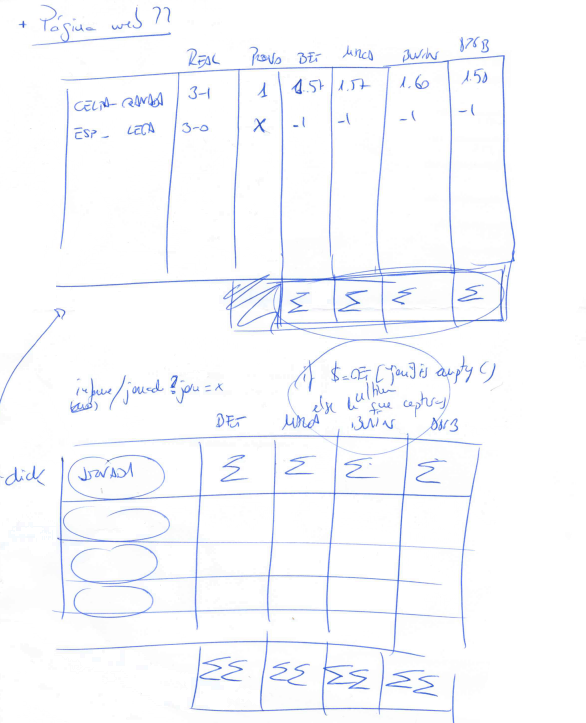
\includegraphics[width=.9\textwidth]{img/prototipo}
\caption{Prototipos diseño web.}
\label{fig:prototipo}
\end{figure}

\begin{figure}
\centering
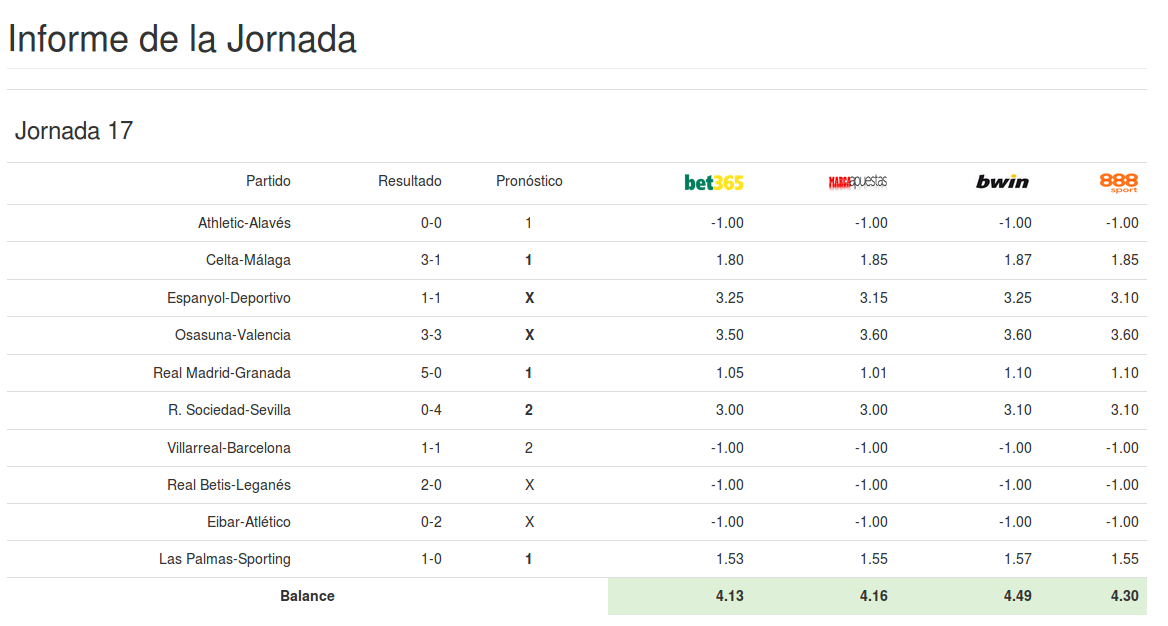
\includegraphics[width=.9\textwidth]{img/drupal_inf_jornada}
\caption{Ventana Informe Jornada.}
\label{fig:infJor}
\end{figure}

\begin{figure}
\centering
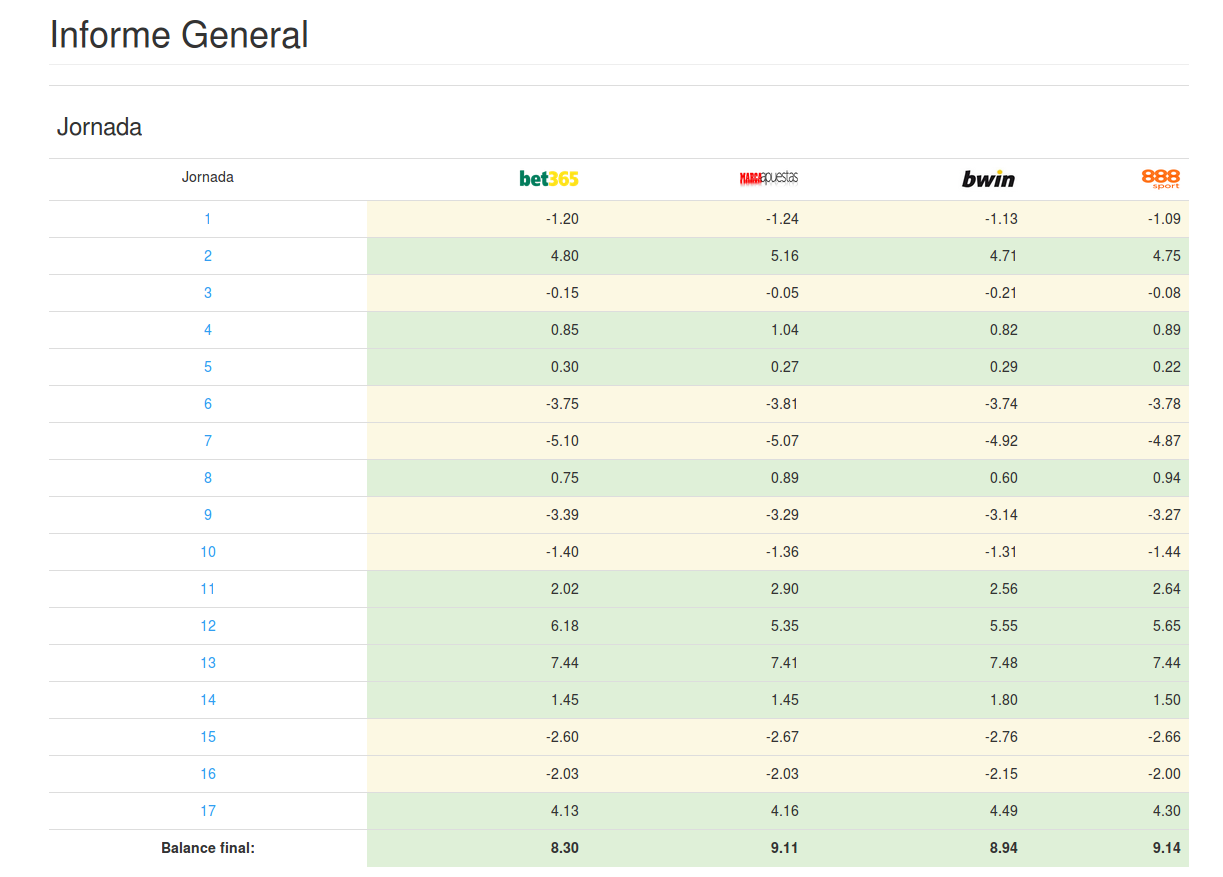
\includegraphics[width=.9\textwidth]{img/drupal_inf_general_usuario}
\caption{Ventana Informe General.}
\label{fig:infGen}
\end{figure}

\section{Automatización del funcionamiento}

Dado que la obtención de datos debe hacerse periódicamente y la ejecución manual por parte del usuario es tediosa, se ha automatizado la ejecución de todos los algoritmos en base al momento en el que deban ejecutarse. Por ejemplo, solo es posible obtener los resultados de una jornada una vez finalizada esta, o es posible fijarse en las cuotas de las casas de apuestas, las cuales pueden ir variando a lo largo de la semana debido a que no son valores fijos.

Para cada jornada se establece una fecha\_antes y una fecha\_despues, los algoritmos de scraping de resultados se ejecutan una vez finalizada la jornada, es decir, si son posteriores a fecha\_despues, algo similar ocurre con el scraping de casas de apuestas solo que en este caso lo mejor es obtener los datos justo antes de la jornada para tener los datos más recientes. Para el algoritmo de backpropagation no es necesario el día exacto en el que ejecutarse, pero debe ejecutarse siempre una vez finalizada la jornada anterior, ya que son necesarias las rachas y los datos de la pasada jornada.

Todo esto lo logramos gracias al uso de demonios, también llamados servicios, que comparan la fecha actual a la fecha de la jornada, ya sea la anterior o posterior, y en caso de coincidir ejecutan el algoritmo deseado. El demonio se ejecuta todos los dias a la misma hora esto se debe a que no todas las jornadas comienzan el viernes y acaban el Lunes si no que algunas jornadas se disputan entre semana.